\documentclass{book}

\usepackage[printonlyused]{acronym}
\usepackage{hyperref}
\usepackage{glossaries}
\usepackage[utf8]{inputenc}
\usepackage{enumitem}
\usepackage{graphicx}
\usepackage{geometry}

\renewcommand{\contentsname}{Sumari}
\renewcommand{\listtablename}{Llista de taules}
\renewcommand{\figurename}{Figura}
\renewcommand{\tablename}{Taula} 

\title{Titol}
\author{Arnau Villoro Bort}

\makeglossaries

%------------------------------------------------------------------
\begin{document}
\frontmatter

\maketitle

\chapter*{Resum} \label{sec:Resum}
\addcontentsline{toc}{chapter}{Resum}
Aquí anirà el resum.

\tableofcontents

\chapter*{Llista d'acrònims}
\label{sec:glossary}
\addcontentsline{toc}{chapter}{Glossari}

%INFO: http://en.wikibooks.org/wiki/LaTeX/Glossary

\begin{acronym}
\acro{PFC}{Projecte Final de Carrera}
\acro{UX}{User Experience}
\acro{UI}{User Interface}
\acro{CSV}{Comma-Separated Values}
\acro{WAAD}{Work Activity Affinity Diagram}
\end{acronym}




\newglossaryentry{smartphone}
{
name = \textit{smartphone}, description = Telefon intel·ligent que permeten realitzar tasques semblants a les realitzades per ordinadors 
}

\newglossaryentry{Android}
{
name = Android, description = Sistema operatiu mòbil amb el qual funcionen la majoria de telèfons mòbils \cite{Android_OS}
}

\newglossaryentry{Google_play}
{
name = Google Play, description = Botiga virtual de Google en la qual es troben les aplicacions per a dispositius mòbils que funcionen amb \gls{Android} (\url{https://play.google.com/store/apps})
}

\newglossaryentry{Holo}
{
name = Holo, description = són unes directrius de disseny per a les aplicacions d'\gls{Android} que es van crear amb la versió 4.0
}

\newglossaryentry{Material}
{
name = Material Design, description = són unes directrius de disseny per a les aplicacions d'Android que es van crear amb la versió 5.0 per a substituir i millorar Holo. Per més informació \url{http://developer.android.com/design/material/index.html}
}

\newglossaryentry{workActivityNotes}
{
name = nota d'activitats de treball, plural = notes d'activitats de treball, description = es tracta de notes que parafrasegen i representen la opinió d'un usuari per a facilitar la comprensió de la opinió dels usuaris.  
}

\printglossary


\chapter*{Apps}
\label{sec:apps}

\begin{enumerate}[label=\bfseries App \arabic*]
  \item \href{https://play.google.com/store/apps/details?id=com.expensemanager}{Expense Manager (Bishinews)} \label{app:ExpenseManager1}
  \item \href{https://play.google.com/store/apps/details?id=at.markushi.expensemanager}{Expense Manager (Markus Hinterseiner)} \label{app:ExpenseManager2}
  \item \href{https://play.google.com/store/apps/details?id=com.bruno.myapps.droidwallet}{Droid Wallet} \label{app:DroidWallet}
  \item \href{https://play.google.com/store/apps/details?id=com.code44.finance}{Financius - Expense Manager} \label{app:Financius}
  \item \href{https://play.google.com/store/apps/details?id=com.handyapps.expenseiq}{Expense IQ} \label{app:Expense IQ}
  \item \href{https://play.google.com/store/apps/details?id=com.techahead.ExpenseManager}{Diario Gasto Gerente (Daily Expense Manager)} \label{app:DailyExpenseManager}
  \item \href{https://play.google.com/store/apps/details?id=com.bookmark.money}{Money lover - Expense Manager} \label{app:MoneyLover}
  \item \href{https://play.google.com/store/apps/details?id=com.kpmoney.android}{AndroMoney (Expense Track)} \label{app:AndroMoney}
  \item \href{https://play.google.com/store/apps/details?id=ru.orangesoftware.financisto}{Financisto} \label{app:Financisto}
  \item \href{https://play.google.com/store/apps/details?id=cz.destil.settleup}{Settle up} \label{app:SettleUp}
  \item \href{https://play.google.com/store/apps/details?id=com.Splitwise.SplitwiseMobile}{Splitwise} \label{Splitwise}
\end{enumerate}
\chapter{Prefaci} \label{Prefaci}

\section{Origen del projecte} \label{OrigenDelProjecte}
Des que tinc memòria he estat molt interessat en la gestió de la informació i de les dades, així com l'enregistrament d'aquestes. No és estrany doncs, el meu interès per a gestionar i controlar les meves despeses. Amb l'aparició dels \glspl{smartphone}, o telèfons intel·ligents, portar un registre de despeses va passar a ser quelcom bastant fàcil. Només calia descarregar-se una aplicació per al mòbil i amb aquesta podies fàcilment apuntar totes les despeses. 

Més endavant vaig descobrir que també hi havia aplicacions que permetien dividir fàcilment les despeses fetes en grup, per a gestionar, per exemple, un viatge amb els amics. Però amb el temps em vaig adonar que, tot i provar-ne moltes, no hi havia cap aplicació que satisfés les meves necessitats. Va ser per això que, cap al Octubre del 2013, vaig decidir que havia de crear jo la meva aplicació.

El problema va ser que en aquell moment em faltaven molts coneixements, però el que em mancava, ho compensava amb moltes ganes i il·lusió. Mig any després i amb moltes hores invertides, ja havia aprés a usar el llenguatge Java, així com a fer aplicacions per a \gls{Android}. 

Paral·lelament vaig començar a buscar idees sobre que podia fer el meu \ac{PFC}. Fins que un bon dia vaig veure unes propostes del Sergi (el meu tutor del \ac{PFC}) a la borsa de projectes, sobre coses relacionades amb \gls{Android} i aplicacions, i que estava obert a propostes. 

A partir d'aquí només va caldre una reunió per a entendre'ns, i així va ser com vam començar aquest projecte. 


\subsection{Motivació} \label{Motivacio}





\mainmatter
\chapter{Introducció}

\section{Objectius del projecte}
L'objectiu d'aquest \ac{PFC} és fer un estudi de l'\ac{UX} per una aplicació que serveixi per a gestionar les despeses personals domèstiques. Amb aquest estudi es pretén arribar a definir com ha de ser aquesta aplicació per a que garanteixi una bona \ac{UX}. I un cop definida com ha de ser, se'n faran proves de concepte basades en aquesta definició. 

Concretament es busca dissenyar una aplicació que:
\begin{itemize}
\item Permeti enregistrar despeses i ingressos tot categoritzant-los.
\item Serveixi per a recordar els deutes (positius o negatius) que es tenen amb diverses persones.
\item Faciliti la gestió de despeses grupals alhora que permeti saldar els deutes minimitzant les transaccions entre els membres.
\item Permeti exportar/importar les dades, tant per a fer còpies de seguretat com per si l'usuari vol utilitzar-les externament.
\item Sigui intuïtiva i senzilla de fer servir.
\item Visualment sigui agradable i minimalista per a que sigui agradable i còmode per a l'usuari.
\end{itemize}

\section{Abast del projecte}
En aquest projecte s'estudiarà l'\ac{UX} per a l'aplicació esmentada tot definint quines utilitats i funcionalitats ha de tenir l'aplicació i com ha de ser la \ac{UI}. L'estudi s'enfocarà únicament en una aplicació per a dispositius mòbils que funcionen amb \gls{Android}, l'actual sistema operatiu més utilitzat\cite{Android_OS} en \glspl{smartphone} o telèfons intel·ligents. 
Finalment en quan al desenvolupament de l'aplicació, no es considera factible crear-la sencera amb totes els requeriments que es dedueixin amb l'estudi de l'\ac{UX}. És per això que es faran proves de concepte intentant apropar-se el màxim possible a com hauria de ser l'aplicació. 

\chapter{Experiència d'Usuari}
\section{Que s'entén per Experiència d'Usuari}
Segons Rex Hartson (2012, p. 19)\cite{UX_Book}, l'\ac{UX} és la totalitat de l'efecte o efectes que sent (o experimenta) internament l'usuari com a resultat de la interacció, i del context d'ús, amb el sistema, dispositiu o producte. És a dir, una bona \ac{UX} es produirà quan l'usuari gaudeixi interaccionant i utilitzant el dispositiu o producte. Interacció i ús s'empren en un sentit molt ampli, ja que inclouen veure, tocar, pensar sobre el producte/dispositiu o fins i tot admirar-lo. 
A més, l'\ac{UX} també engloba la usabilitat i la utilitat. Certament l'usuari sent internament parts de la usabilitat, com l'augment de productivitat, però hi ha certes manifestacions de usabilitat, com podria ser el temps invertit en la tasca, que representa un component no necessàriament experimentat internament per l'usuari.

\section{Com s'estudia l'Experiència d'Usuari?}
L'\ac{UX} no pot ser dissenyada ja que depèn, no només del producte en si mateix, sinó que també depèn de l'usuari i la situació en la que l'utilitza [Smashing Magazine, 2012, p. 25-28]\cite{Smashing_User_Experience_Design}. I és que no és possible dissenyar ni l'usuari ni la situació. Però el que si es pot fer és dissenyar per a una bona \ac{UX} i és això el que s'entén per fer un estudi d'\ac{UX}. Per a fer-ho es segurian les 4 activitats elementals o etapes que Rex Harton proposa en el seu llibre d'\ac{UX} \cite{UX_Book}, que són anàlisi, disseny, implementació i avaluació, tal i com es pot veure a la figura \ref{fig:UX_lifecycle}. Per tal d'aconseguir proporcionar una bona \ac{UX} aquestes activitats és duen a terme de forma iterativa, ja que no sempre és possible trobar un bon disseny al primer intent.

\begin{figure}[htp]
\centering
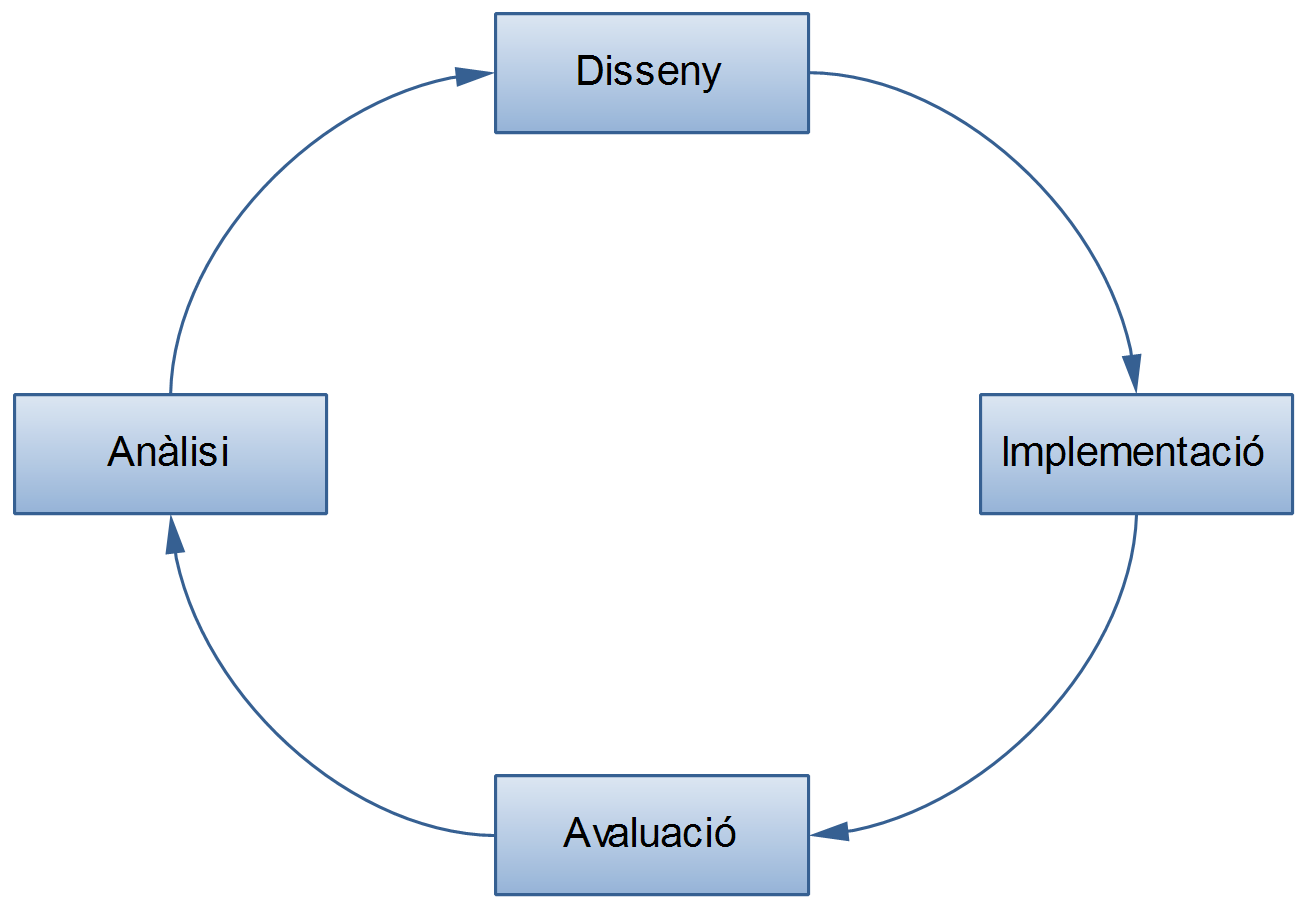
\includegraphics[scale=0.6]{UX_wheel.png}
\caption{Activitats a seguir per a dissenyar garantint una bona \ac{UX}}\label{fig:UX_lifecycle}
\end{figure}

Aquestes quatre activitats, a grans trets, consisteixen en:
\begin{description}
\item [Anàlisi] Es basa en entendre les necessitats de l'usuari que utilitzarà el producte.
\item [Disseny] Consisteix en la creació de dissenys conceptuals determinant la interacció, el comportament i l'aparença del producte.
\item [Implementació] Correspon a la creació de prototips.
\item [Avaluació] Es tracta de comprovar si el disseny satisfà les necessitats dels usuaris que s'han determinat.
\end{description}

\subsection{Anàlisi}\label{sec:analisi}
L'objectiu general d'aquesta activitat és definir com són les usuaris potencials. Un cop definits, serviran per a poder extreure com interaccionaran amb el producte, quines necessitats tindran i en conseqüència els requeriments del producte, tal com afirma Rich Fulcher \cite{user_centred_design}.

Dins de l'anàlisi hi ha quatre subactivitats o passos a seguir:

\subsubsection{Investigació contextual}\label{subsec:investigacio_contextual}
Durant la investigació contextual s'estudia com les persones treballen o interactuen amb el producte en el seu entorn de treball. Per treball s'entén l'ús del producte en si i per entorn de treball, l'entorn en que habitualment s'usa aquest. S'utilitzen aquests termes independentment de la tipologia del producte. És a dir, encara que el producte fos un joc, al fet d'utilitzar-lo se l'anomena treballar. 

Durant la investigació contextual es tracta d'investigar i descobrir com l'usuari treballa en l'entorn habitual i això no es pot determinar enquestant als usuaris. El problema és que la descripció que pugi fer un usuari de com treballa no és fiable. La forma correcta d'investigar és observant com els usuaris treballen i entrevistant-los mentre ells duen a terme aquesta activitat. Per tant es tracta de:

\begin{itemize}
\item Preparar i realitzar visites de camp a l'entorn de treball, on el producte serà utilitzat, de l'usuari/client.
\item Observar i entrevistar els usuaris mentre treballen.
\item Indagar en l'estructura de la pròpia pràctica de treball de l'usuari.
\item Aprendre com la gent treballa en l'entorn en el qual treballarà amb el producte a dissenyar.
\item Extreure notes detallades de les observacions i entrevistes.
\end{itemize}

Durant la investigació contextual és important no preguntar als usuaris que volen o necessiten. En aquesta etapa no es busca que necessiten sinó observar i entrevistar els usuaris en el seu entorn de treball sobre com treballen.


\subsubsection{Anàlisi contextual}\label{subsec:analisi_contextual}
L'essència d'aquest pas és el processament, la interpretació i l'anàlisi de la informació aconseguida a la investigació contextual (apartat \ref{subsec:investigacio_contextual}). Això s'aconsegueix a base de:

\begin{itemize}
\item Crear un model de flux.
\item Sintetitzar la informació en \glspl{workActivityNotes}.
\item Construir un \ac{WAAD} a partir de les \glspl{workActivityNotes}.
\end{itemize}

El model de flux és una representació gràfica que explica com les diferents entitats es comuniquen per tal d'aconseguir que el treball es realitzi. Per a poder crear el model de flux cal identificar els rols de treball. Un rol de treball correspon als deures, funcions i activitats que desenvolupa una persona amb cert lloc de treball.

\begin{figure}[htp]
\centering
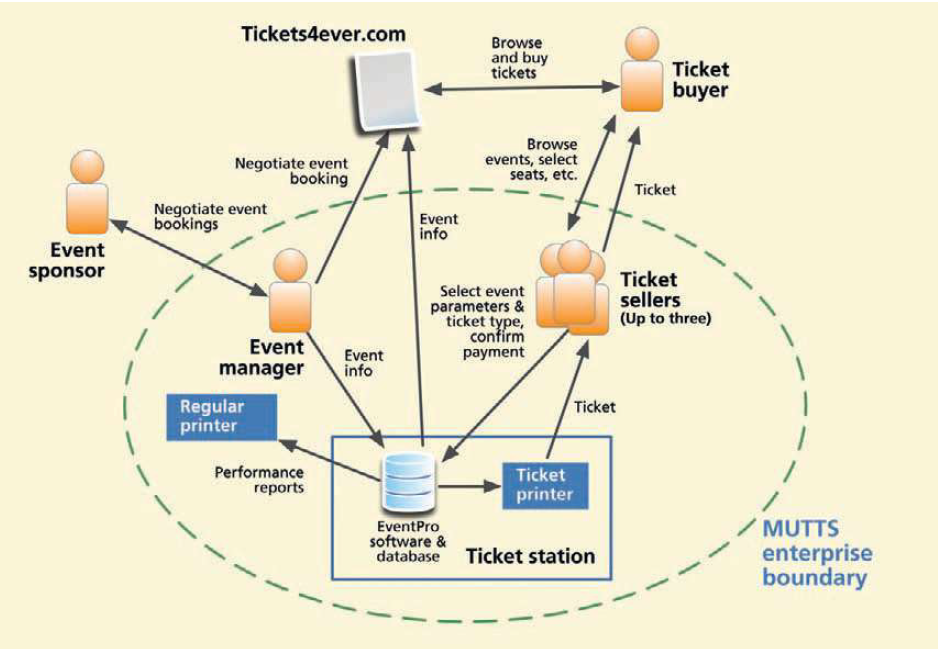
\includegraphics[scale=0.6]{flow_model_example.png}
\caption{Exemple de model de flux.}\label{fig:flow_model_example}
\end{figure}

Paral·lelament a la creació del model de flux, cal sintetitzar la informació en brut que s'ha extret a la investigació contextual. Això es fa creant \glspl{workActivityNotes} les quals, un cop tota la informació ha estat processada, han de representar tota la informació abans extreta. Aquestes notes es caracteritzen per estar escrites en primera persona (des de la perspectiva de l'usuari) parafrasejant i sintetitzant la opinió d'aquest. Cada nota ha de ser concisa i compacta, de manera que expressi una sola idea. Un exemple d'aquestes notes és el de la figura \ref{fig:workActivityNote1}. Com es pot veure cal etiquetar les notes amb un identificador representant l'usuari del qual provenen.

\begin{figure}[htp]
\centering
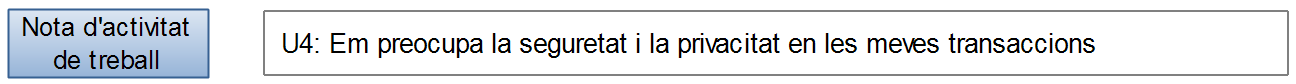
\includegraphics[scale=0.3]{WorkActivityNotes1.png}
\caption{Exemple d'una nota d'activitats de treball}\label{fig:workActivityNote1}
\end{figure}

Les \glspl{workActivityNotes} serveixen per a construir el \ac{WAAD}. Aquest diagrama consisteix en l'agrupació de les notes segons grups o afinitats segons la perspectiva de l'usuari. L'objectiu d'aquest diagrama és transmetre de forma clara i ràpida la opinió dels usuaris. El que es busca es que ja no sigui necessari llegir les llargues transcripcions de la investigació contextual ja que el \ac{WAAD} n'és una representació d'aquesta. 

\subsubsection{Extracció dels requeriments d'interacció}\label{subsubsec:Extraccio_requeriments}
La idea general d'aquesta etapa es recórrer l'estructura jeràrquica del \ac{WAAD} per extreure sentencies sobre els requeriments del sistema. Això és dur a terme analitzant les \glspl{workActivityNotes} per deduir les necessitats i/o requeriments que cada nota implica. Els requeriments que s'extreuen s'han d'etiquetar per categories (i subcategories si fa falta) juntament amb un identificador que els relacioni amb la \gls{workActivityNotes} de la qual prové. Així si en un anàlisi posterior sorgeixen dubtes, es pot buscar la font de cada requeriment. 

És també important extreure aquells requeriments que l'usuari considera obvis i que per tant no menciona ni descriu i que per tant no estan implícitament a les \glspl{workActivityNotes}.

\begin{figure}[htp]
\centering
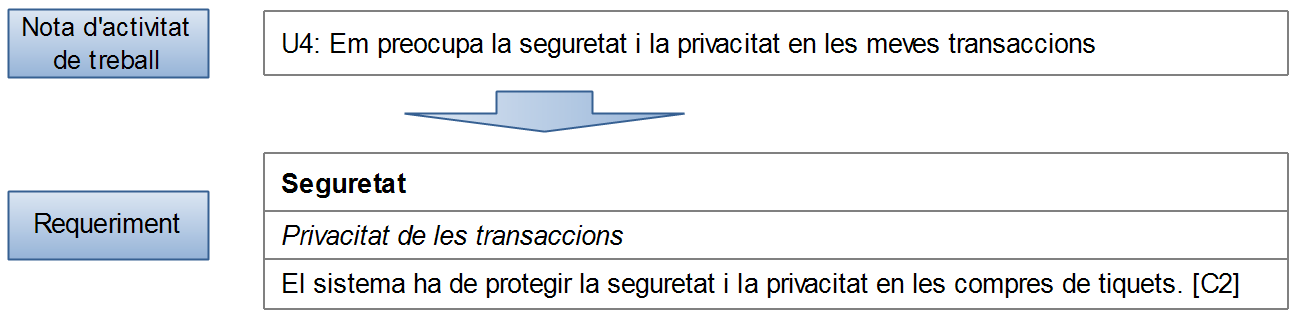
\includegraphics[scale=0.3]{WorkActivityNotes2.png}
\caption{Documents resultants de l'extracció de requeriments}\label{fig:workActivityNote2}
\end{figure}

A la figura \ref{fig:workActivityNote2} es pot veure com s'extreu un requeriment, utilitzant el mateix exemple que abans (figura \ref{fig:workActivityNote1}). L'etiqueta "C2", fa referencia a la posició que ocupava la nota dins el \ac{WAAD}. S'utilitzen les lletres per anomenar les diferents branques i sub-branques i els números per diferenciar les notes que hi ha la mateixa branca del \ac{WAAD}.

Un cop generats els requeriments es comprovarà que aquests siguin correctes preguntant directament als usuaris. Sempre que sigui possible es preguntarà als usuaris que van participar en la investigació contextual (apartat \ref{subsec:investigacio_contextual} juntament amb d'altres nous usuaris. Aquest pas també pot servir perquè els usuaris ajudin a destacar aquells requeriments que són prioritaris.

\subsubsection{Construcció de models informatius per al disseny}\label{subsubsec:Construccio_models}
Per dur a terme aquesta etapa també cal recórrer el \ac{WAAD}, és per això que aquesta etapa no és posterior a l'etapa \ref{subsubsec:Extraccio_requeriments} sinó que les dues es duen a terme de forma paral·lela. L'objectiu d'aquesta etapa és obtenir una sèrie de documents que descriuen tant el sistema actual, com el sistema que es preveu. Aquests documents seran els que es faran servir per a dissenyar el nou producte.

Aquest pas, juntament amb l'anterior (apartat \ref{subsec:analisi_contextual}) serveixen de pont entre l'anàlisi en si i l'etapa del disseny. És a dir, serveixen per enllaçar la situació o model actual, amb el model o sistema que s'està dissenyant.

Els documents que s'obtenen en aquesta etapa (figura \ref{fig:design-informing_models}) són: 
\begin{figure}[ht]
\centering
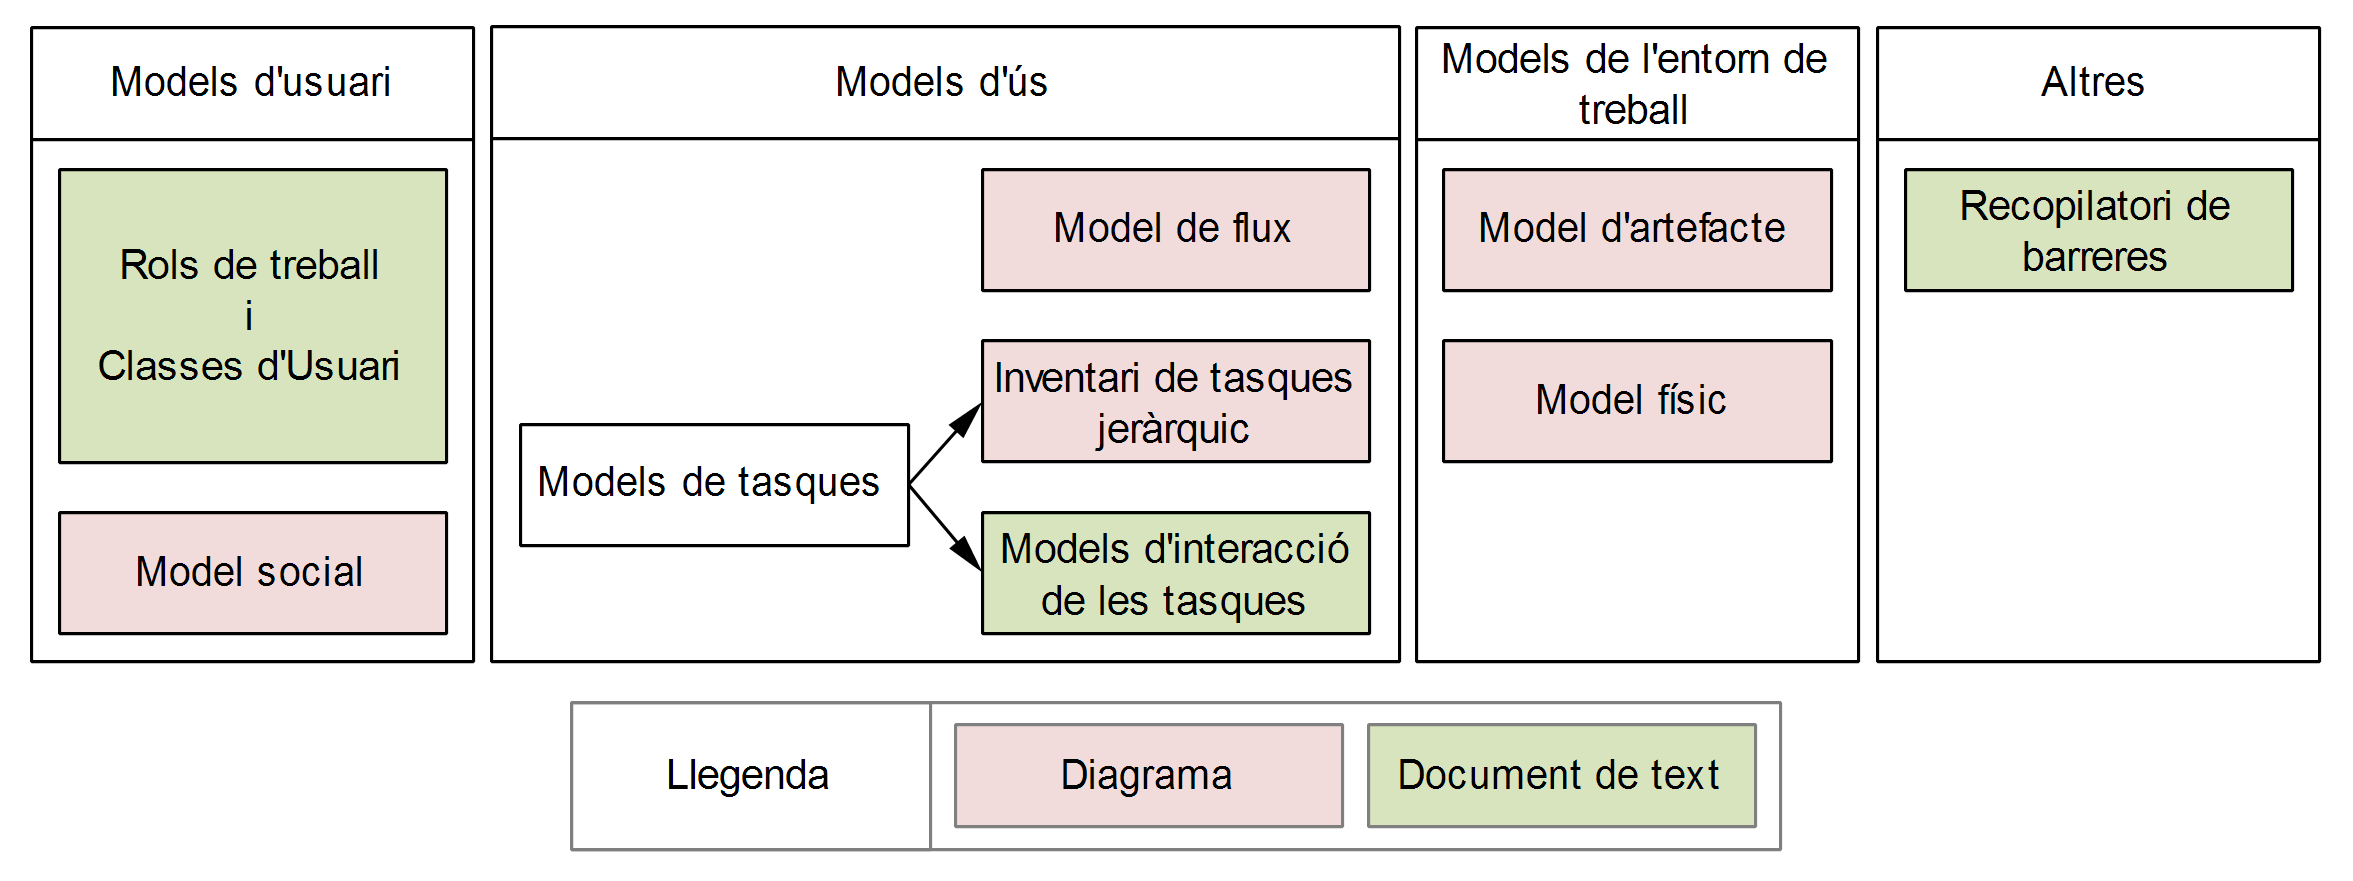
\includegraphics[scale=0.75]{Design-informing_models.png}
\caption{Exemple d'extracció de requeriments}\label{fig:design-informing_models}
\end{figure}

\begin{description}
\item[Rols de treball] Corresponen als deures, funcions i activitats que desenvolupa una persona amb cert lloc de treball.
\item[Classes d'Usuaris] Són les diferents característiques de la gent que desenvolupa un rol de treball concret.
\item[Model social] És un diagrama que mostra l'organització i relació que existeix entre les diferents persones que intervenen en el sistema.
\item[Model de flux] Aquest diagrama mostra com les diferents entitats (ja siguin, persones, aparells o programes) interaccionen entre si i què intercanvien entre elles.
\item[Inventari de tasques jeràrquic] Es tracta d'un inventari jeràrquic que mostra les diferents tasques que es poden executar en el sistema.
\item[Models d'interacció de les tasques] És un document que detalla com es duen a terme les tasques i com interaccionen les entitats que intervenen (sempre que intervingui més d'una entitat).
\item[Model d'artefacte] Aquest diagrama mostra com els diferents elements tangibles interactuen entre si.
\item[Model físic] Aquest model mostra la distribució física dels diferents artefactes i entitats.
\item[Recopilatori de barreres] És un recopilatori de les barreres que s'han descrit als documents anteriors.
\end{description}

Una barrera és un problema que interfereix amb les operacions que l'usuari executa normalment. És qualsevol cosa que impedeix l'activitat de l'usuari, interromp el flux habitual del treball o interfereix amb el desenvolupament del treball. Seguint les recomanacions de Rex Harton (2012, p. 186) \cite{UX_Book} habitualment s'utilitza la mateixa simbologia que Beyer i Holtzblatt \cite{Contextual_Design} per a representar les barreres (el llamp vermell \barrier)

\subsection{Disseny}
Aquest pas consisteix en crear diversos dissenys conceptuals que mostren com serà el producte que es busca crear, determinant com ha de ser la interacció amb aquest i la seva aparença. 

Al dissenyar és important saber per a quin tipus d'usuari es dissenya. I és que tal com diu Cooper (2004, p. 124) \cite{Cooper} no és possible crear un disseny que funcioni per a tothom i és millor tenir un petit percentatge de la població completament satisfeta que no pas tota la població mig satisfeta. Afirma que fins i tot és preferible tenir un percentatge més petit de la població extasiada amb el producte. Per a facilitar que en aquesta etapa es dissenyi per a satisfer totes les necessitats de cert grup de la població, cal crear personatges, creant un personatge per a cada rol definit prèviament. La creació d'aquests personatges és un pas clau per a aconseguir crear un bon producte. Per a crear cada personatge primer es creen personatges a partir dels usuaris que han intervingut a l'anàlisi. Després es fusionen els personatges que tenen les mateixes metes. Ara, d'entre els personatges que queden, cal escollir aquell personatge que, si es dissenya exclusivament per a ell, el producte funcionarà prou bé per la resta de persones. Si cal s'agafaran característiques de diferents personatges per a crear el personatge definitiu. 

Un cop es tenen els personatges creats, comença la part del disseny en si. Aquí Rex (2012, p. 335) \cite{UX_Book} proposa fer 5 passos on cada cop es refina més el disseny, fins a assolir el disseny definitiu. Aquestes etapes són:

\begin{itemize}
\item Ideació i esbossos
\item Disseny conceptual
\item Disseny intermedi
\item Disseny detallat
\item Refinat del disseny
\end{itemize}


\subsubsection{Ideació i esbossos}
Aquest primer pas consisteix en explorar idees. Per una banda amb la ideació, és a dir, el procés de formar idees per el disseny, la qual cosa normalment és fa amb una pluja d'idees. Per l'altre es creen esbossos per a plasmar les idees d'alguna de les persones que està dissenyant. Es important remarcar que les idees o esbossos que es creen en aquest pas han de tenir un nivell de detall molt baix. El que es busca és un primer contacte amb les idees, per tant és important deixa llibertat per a que sorgeixin el màxim d'idees, sense limitar-les a si semblen factibles o no. 

\subsubsection{Disseny conceptual}
Per \gls{conceptual_design} s'entén, un tema, noció o idea amb el propòsit de comunicar una visió del disseny del sistema o producte. És la part del disseny del sistema que porta el model mental del dissenyador a la vida. 
Aquí es busca avaluar i comparar diversos dissenys conceptuals mirant també la seva viabilitat. 

\subsubsection{Disseny intermedi}
L'objectiu del disseny intermedi és crear la navegació, estructura i disseny de les pantalles, amb un nivell de fidelitat mitjà. Parteix dels dissenys conceptuals i es busca descomposar-los en unitats lògiques, expandint-les en diferents possibilitats de disseny. 

En el disseny intermedi és defineix completament com ha de ser la navegació. Tot i això el contingut de cada apartat o pàgina només es mostra de forma aproximada, amb un nivell de fidelitat mitjà, sense masses detalls. 
És en aquesta etapa on prenen màxima rellevància els documents que s'han obtingut en l'etapa de construcció de models informatius \ref{subsubsec:Construccio_models}.

\subsubsection{Disseny detallat}
En aquest pas es busca detallar el disseny. Aquí es defineix completament l'aparença de tots els elements que apareixen en pantalla, definint els objectes que els formen, colors, mides, fonts, marges i localització de cada un d'ells. A la figura \ref{fig:design_Sunshine} es pot veure un exemple de disseny detallat d'una aplicació per \gls{Android}.

\begin{figure}[ht]
\centering
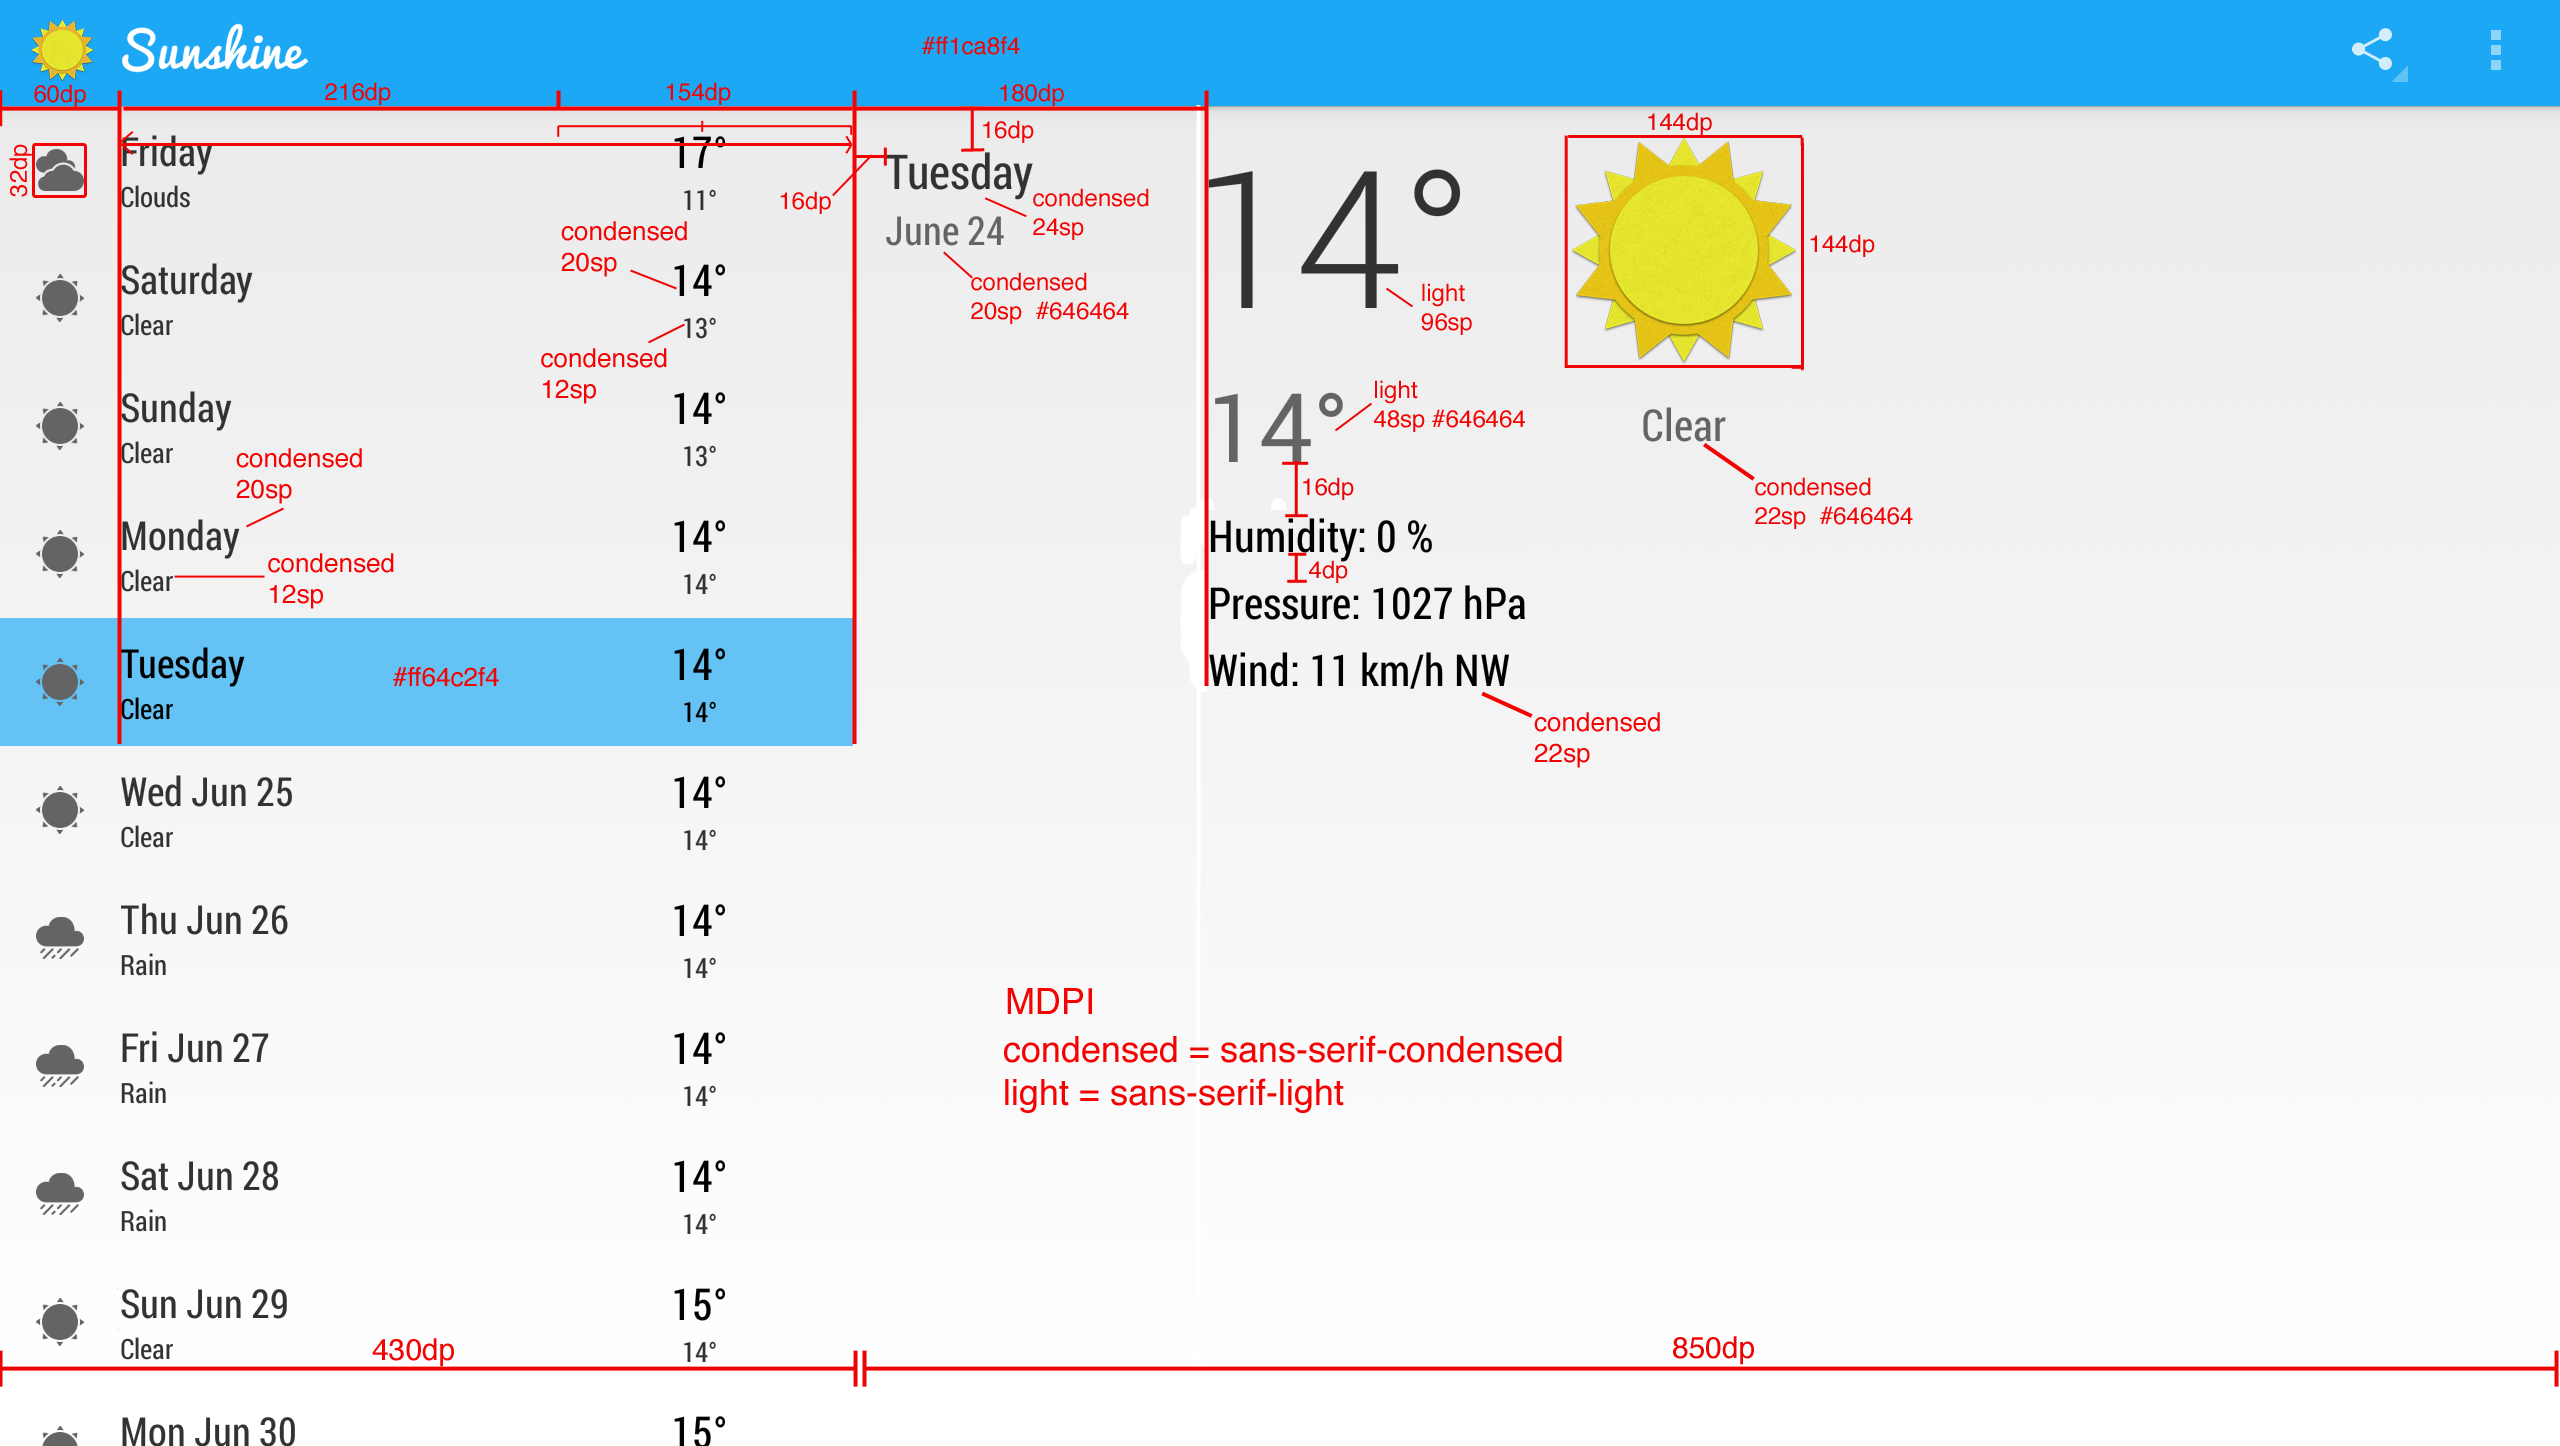
\includegraphics[scale=0.17]{Sunshine_detailed_design.png}
\caption{Exemple de disseny detallat. Font: Udacity (Developing Android Apps) \cite{developing_android_apps}}
\label{fig:design_Sunshine}
\end{figure}

\subsubsection{Refinat del disseny}
Aquesta etapa es centra a buscar i arreglar problemes de \ac{UX} 


%TODO HEX proposa que s'adaptin els metodes als recursos disponibles
\subsection{Implementació}\label{subsec:implementation}
En la implementació o prototipatge es busca poder avaluar amb els usuaris els dissenys que s'han creat i es du a terme mitjançant prototips, els quals són representacions navegables del producte final. Tal com Nielsen (1993) \cite{Nielsen_1993} proposa, els prototips es poden classificar segons la funcionalitat i segons les funcions o característiques que implementen, tal com es veu a la figura \ref{fig:types_prototypes}. També defineix els prototips horitzontals, verticals i locals. Aquests es caracteritzen per:

\begin{figure}[ht]
\centering
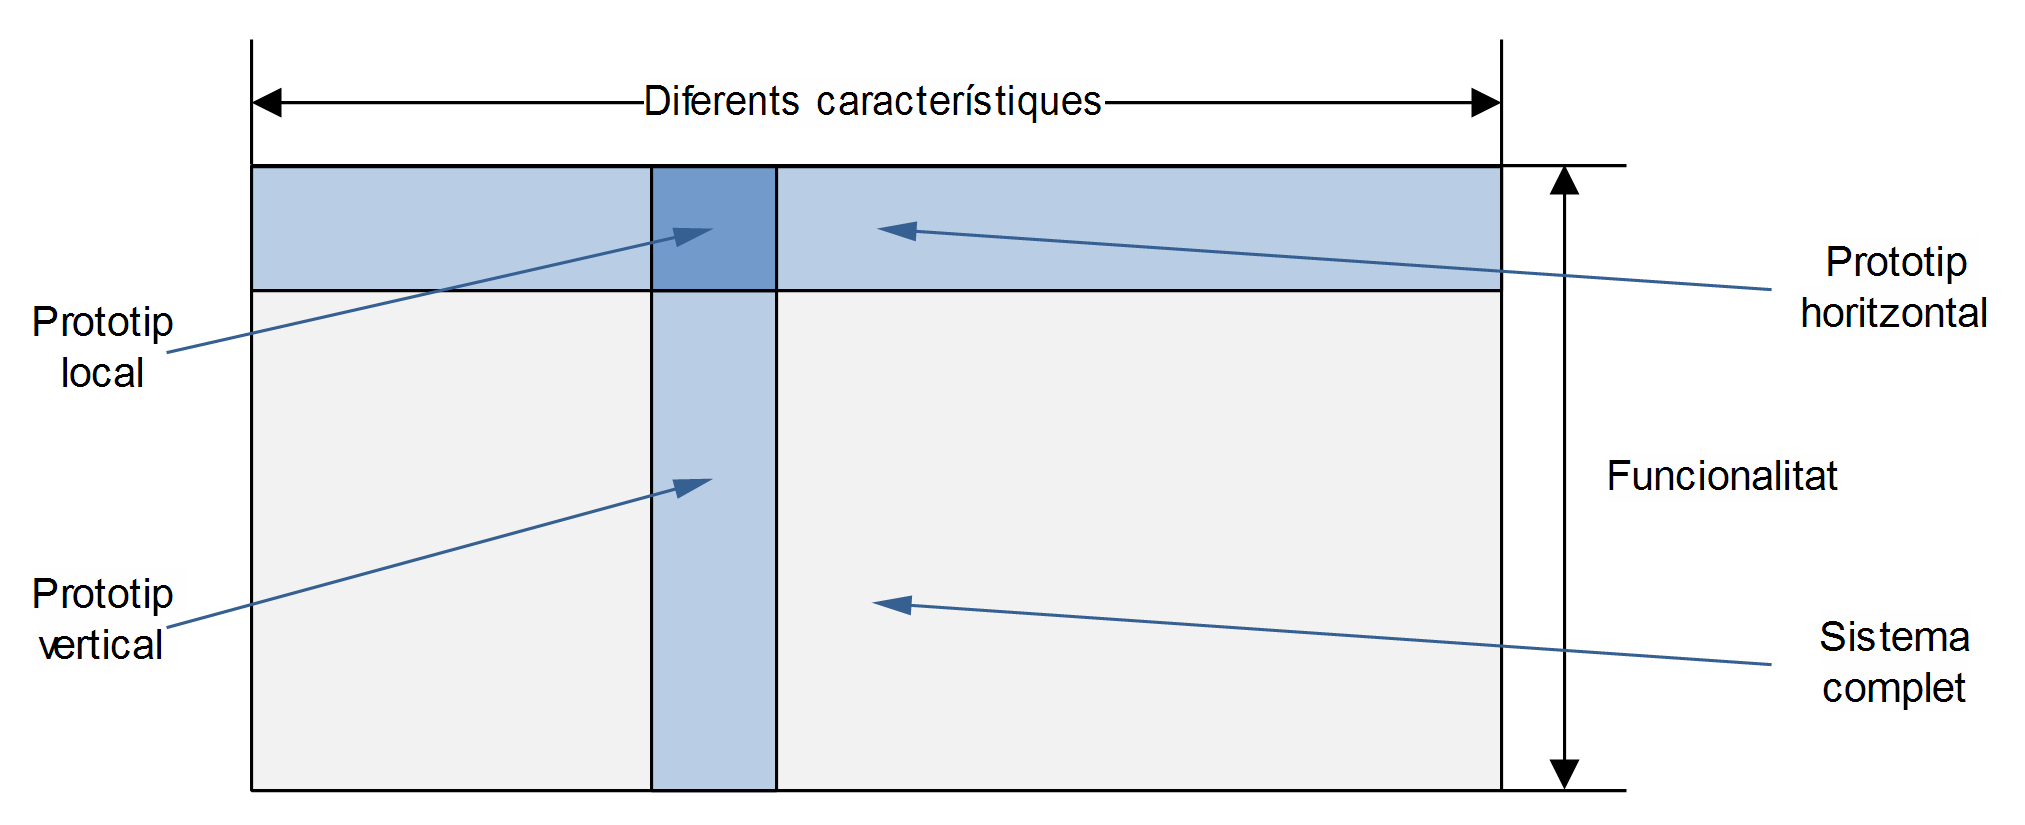
\includegraphics[scale=0.8]{Types_prototypes.png}
\caption{Tipus de prototips}\label{fig:types_prototypes}
\end{figure}

\begin{description}
\item[Prototip Horitzontal] És caracteritza per tenir moltes funcions però amb una profunditat molt baixa de funcionalitat. Serveix per a demostrar les diferents característiques o funcions que tindrà el producte, de manera que es pot veure de forma general les seccions o apartats i la navegació en general.
\item[Prototip Vertical] Aquest tipus de prototip té una profunditat màxima de funcionalitat però centrat només en unes poques funcions. S'utilitza per avaluar amb suficient detall algunes funcions concretes del producte. 
\item[Prototip Local] És un tipus de prototip on només implementa unes poques funcions i amb poca profunditat en quan a funcionalitat. S'utilitzen per avaluar diferents alternatives de disseny per a certs detalls d'interacció amb el sistema. 
\end{description}

Els prototips també es poden classificar segons el nivell de fidelitat, és a dir, com de "finalitzat" percep l'usuari el prototip. Es classifiquen doncs en baixa, mitja o alta fidelitat. 

\begin{description}
\item[Prototips de baixa fidelitat] Aquests prototips s'utilitzen en les primeres etapes de disseny, ja que impliquen poca feina i per tant són senzills de modificar. Aquest tipus de prototips habitualment es fan dibuixant amb paper i bolígraf. 
\item[Prototips de mitja fidelitat] Es tracta d'un terme mig entre prototip de baixa i el d'alta fidelitat. Tot i que no representen l'aspecte final del producte, si s'acosten donant una idea més real de com serà. Aquests tipus de prototips normalment es creen amb programes especials per a ordinadors.
\item[Prototips d'alta fidelitat] Els prototips d'alta fidelitat tenen un aspecte i comportament molt realista i pròxim al producte final. S'utilitzen per a polir i refinar el disseny del producte. 
\end{description}

Quan menys fidel és un prototip, és alhora més susceptible de canviar. I és que un prototip de baixa fidelitat és percebut com a poc fidel al producte final per un usuari, i com a conseqüència, desinhibeix als usuaris a l'hora de criticar-lo i aportar idees per a millorar-lo. En canvi, en un prototip d'alta fidelitat, al ser tant pròxim al producte final, l'usuari percep que hi ha molta feina darrere d'aquest i que per tant és complicat modificar-lo i això portarà a que tendeixi a no criticar-lo, amb la idea de no menystenir la feina d'altres persones. Tot i això, els prototips de baixa fidelitat són complicats d'entendre per les persones que no estan familiaritzades, per això és recomanable que només s'utilitzin i es comparteixin amb l'equip de disseny i, si existeixen, amb usuaris que estiguin familiaritzats amb el procés de disseny. Per tant, de forma general, els prototips de mitja fidelitat són els primers que es comparteixen amb els usuaris. 


Els prototips són representacions navegables que exemplifiquen com serà el producte o sistema. Com a tals, hi ha varies maneres d'aconseguir que siguin navegables, permetent més o menys interacció. Es tenen doncs:

\begin{description}
\item[Prototips de paper] Consisteix en crear en paper els diferents elements del sistema i utilitzar una base per a poder-los mostrar. L'usuari simula clics als diferents elements i l'avaluador far aparèixer els elements necessaris que corresponen a la resposta del clic que ha fet l'usuari. 
\item[Prototips "Mag d'Oz"] Aquests tipus de prototips es basen en dos aparells, un per a l'usuari i un per l'avaluador. L'usuari interactuarà amb el seu dispositiu i l'avaluador, amb l'altre dispositiu rebrà les accions de l'usuari i les respondrà simulant el comportament del sistema.
\item[Prototip completament programat] És un prototip programat que representa de manera bastant fidel el producte/sistema final.
\end{description}

Durant la creació d'un producte el més habitual és començar creant prototips horitzontals de baixa fidelitat per a poder generar una primera impressió del producte. A mesura que es va perfeccionant el producte, es va millorant la fidelitat d'aquest i permetent més interacció de manera que els usuaris notin que interactuen amb prototip molt semblant al producte final. D'aquesta manera s'inverteixen pocs recursos amb els primers prototips ja que són més susceptibles de canviar i un cop es sap que el producte va per el bon camí es quan es creen els prototips d'alta fidelitat, invertint només una quantitat elevada de recursos quan és necessari. 

\subsection{Avaluació}
Per avaluació s'entén validar que el producte compleix les expectatives dels usuaris. Per a fer-ho, hi ha dos tipus d'avaluació, l'avaluació formativa i la sumarial. 

\begin{description}
\item[Avaluació formativa] Es tracta d'un primer diagnostic. Consisteix en recol·lectar informació qualitativa per identificar i arreglar problemes de \ac{UX} i les seves causes en el disseny.
\item[Avaluació sumarial] Consisteix en recol·lectar informació quantitativa per assegurar un nivell de qualitat en un disseny, especialment per a l'avaluació de la millora de la \ac{UX} a causa de l'avaluació formativa. Es dur a terme en les últimes fases de disseny quan els prototips ja tenen una fidelitat alta. 
\end{description}

La informació que s'obté a l'avaluació pot ser objectiva o subjectiva i quantitativa o qualitativa.

\begin{description}
\item[Informació objectiva] Es tracta d'informació observada per l'avaluador o per l'usuari sobre inconsistències o problemes. 
\item[Informació subjectiva] Són les opinions o judicis del usuaris respecte a la seva \ac{UX} i la satisfacció al interactuar amb el producte. 
\item[Informació quantitativa] És la informació numèrica que demostra la qualitat del producte. S'obté a través d'analitzar el rendiment o amb qüestionaris i és la base de l'avaluació sumarial.
\item[Informació qualitativa] És informació descriptiva que normalment descriu problemes d'\ac{UX} observats durant la utilització del producte.
\end{description}

Per a poder recopilar informació a l'hora d'avaluar, Rex (2012, p. 360 - 490) \cite{UX_Book} proposa un seguit de tècniques:

\begin{itemize}
\item Detecció d'incidents crítics
\item Tècnica "pensar en veu alta"
\item Demostració del producte
\item Inspecció 
\item Qüestionaris
\item Versions alfa/beta
\item Mètriques \ac{UX}
\end{itemize}

\subsubsection{Detecció d'incidents crítics}
Un incident crític és un esdeveniment observat durant el desenvolupament de les tasques que ha produït sorpresa, ha molestat o inquietat a l'usuari per la seva falta de coherència o per presentar resultats inesperats per l'usuari. La detecció d'incidents crítics consisteix en analitzar els usuaris mentre utilitzen el producte per a poder trobar-los. És una tècnica d'avaluació formativa que serveix per a recopilar informació qualitativa. Els incidents crítics sovint són expressats verbalment per els usuaris, però a vegades també poden ser expressats de forma no verbal mitjançant unt titubeig, encongiment d'espatlles o alguna ganyota. 
\subsubsection{Tècnica "pensar en veu alta"}
La tècnica "pensar en veu alta" és una tècnica per aconseguir informació qualitativa que, com el seu nom indica, consisteix en què el usuaris expressin verbalment els seus pensaments, els seus motius i la seva percepció sobre els problemes d'\ac{UX} en quan a la interacció amb el producte quan l'estan fent servir. Amb aquesta tècnica s'aconsegueix entendre que és el que l'usuari intenta fer en tot moment i quins problemes experimenta.
És important que els usuaris expliquin què és el que estan pensant, no el que estan fent, ja que això és el que seria més complicat de saber sense fer servir aquesta tècnica.  
\subsubsection{Demostració del producte}
Una demostració o \textit{walkthrough} és un mètode que s'acostuma a fer servir en les primeres etapes de disseny abans que existeixi algun prototip. Consisteix en ensenyar el producte als usuaris fent-se passar per un, de manera que aquests veuran el disseny com si fossin uns experts. La idea és que l'equip intenta anticipar-se als problemes que els usuaris podrien tenir si fossin ells els que estiguessin utilitzant el producte. 
\subsubsection{Inspecció} 
La inspecció consisteix en que un expert en UX provi i avaluï ell mateix el producte enlloc de que el facin servir usuaris mentre l'expert els observa. Per tant, l'avaluador fa alhora d'observador i participant. Aquesta tècnica és útil a les primeres etapes del disseny per a poder trobar els problemes d'\ac{UX} més evidents a un baix cost. 
\subsubsection{Qüestionaris}
Els qüestionaris són la eina principal per a recol·lectar informació objectiva del producte. S'utilitzen principalment com a una eina de formació sumarial. Hi ha molts qüestionaris creats específicament per avaluar l'\ac{UX}, tot i això els més coneguts i d'ús lliure són:
\begin{itemize}
\item Qüestionari per a la satisfacció amb la interfície d'usuari o \textit{Questionnaire for User Interface Satisfaction} (QUIS).
\item Escala d'usabilitat del sistema o \textit{System Usability Scale} (SUS).
\item Utilitat, satisfacció i facilitat d'ús o \textit{Usefulness, Satisfaction and Ease of Use} (USE).
\end{itemize}

\subsubsection{Versions alfa/beta}
Quan el producte és una aplicació de \textit{software} i el procés de desenvolupar-la s'ha acabat és habitual que s'envii primer a certs usuaris, experts, clients i crítics professionals per a que en donin la seva opinió. Una versió alfa és una versió més prematura i menys polida del producte que s'envia a una audiència més reduïda també a l'objectiu d'aconseguir la seva opinió. 
Aquestes versions són una forma gratuïta d'aconseguir les opinions dels usuaris abans de llançar finalment el producte al mercat i serveixen per a comprovar com acollirà el públic el producte. Sovint també serveix per a detectar erros que s'hagin pogut passar per alt al desenvolupar el producte. 

\subsubsection{Mètriques \ac{UX}}
Aquesta tècnica consisteix en establir certs objectius en quan a \ac{UX} que siguin quantificables. Un cop establits, es defineix un valor mínim o cota, normalment amb un producte ja existent. Quan ja es té un valor es tracta de calcular el valor de cada mètrica amb el prototip i veure si és supera la cota. En aquesta tècnica es fan servir les taules de mètriques com per exemple la taula \ref{table:UX_metrics}.

\begin{table}
\begin{tabular}{ | p{2.4cm} | p{2.7cm} | p{2.6cm} | p{1.6cm} | p{2.6cm} |}
\hline
\headB{Objectiu \ac{UX}} & \headB{Mesura \ac{UX}} & \headB{Mètrica \ac{UX}} & \headB{Cota} & \headB{Valor observat} \\
\hline
Facilitat d'ús & Rendiment inicial de l'usuari & Temps mitjà & 3 min. & 2,5 min. \\
\hline
Facilitat d'ús & Rendiment inicial de l'usuari & Nombre mitjà d'errors & $<1$ & $<1$ \\
\hline
\end{tabular}
\caption{Taula exemple de les mètriques \ac{UX}}
\label{table:UX_metrics}
\end{table}


\section{El procés iteratiu}
A l'hora de dissenyar per a una bona \ac{UX} és important fer les quatre activitats fonamentals de forma iterativa per tal d'assegurar que la solució realment és bona. Per tant, quan és fa un estudi d'\ac{UX} és comença amb un anàlisi utilitzant els productes/sistemes semblants al que es vol dissenyar per a veure com els usuaris interactuen amb ell i que n'esperen. Un cop finalitzada l'etapa de l'anàlisi per primer cop, és faran els primers dissenys i s'implementaran fent els primers prototips de baixa fidelitat per no malbaratar recursos. Amb aquests prototips s'avaluarà la idoneïtat de la solució dissenyada i, si s'escau, és corregiran els documents que s'havien aconseguit a l'etapa de l'anàlisi. Un cop s'ha fet la primera iteració, s'anirà fent dissenys cada cop més detallats i implementant prototips de fidelitat més alta. D'aquesta manera s'acabarà arribant a un disseny definitiu i a un prototip que serà molt semblant a com ha de ser el producte final.

Al ser un procés iteratiu pot semblar que a les primeres iteracions no és imprescindible arribà a un disseny i/o prototip bo, ja que en les següents iteracions ja s'aconseguirà que aquests siguin bons. Però a la realitat això no és així, cada iteració implica utilitzar recursos, per tant per a ser eficients és millor no fer masses iteracions. És a dir, des d'un bon principi és busca aconseguir dissenyar garantint la millor \ac{UX} possible.

A la taula \ref{table:UX_sum_up} és mostra un resum aproximat de com és relacionen les diferents etapes entre si. És una representació dels passos que es segueixen durant el procés iteratiu. Tot i que s'ha intentat ordenar cronològicament en funció de l'ordre d'execució, a la realitat és habitual que algunes etapes es solapin o es duguin a terme simultaneïtat, sobretot quan s'estan explorant diversos possibles dissenys.

\begin{table}
\begin{tabular}{ | p{1.8cm} | p{5cm} | p{3cm} | p{3cm} |}
\hline
\headB{Passos del disseny} & \headB{Propòsit} & \headB{Prototip} & \headB{Avaluació} \\
\hline
Ideació i esbossos & Explorar idees de disseny & Esbossos & Discutint i criticant amb l'equip de disseny \\
\hline
Disseny conceptual & Avaluar i comprar múltiples dissenys conceptuals & Prototips de paper i \gls{wireframe} i \textit{storyboards} de baixa fidelitat &  Fent demostracions del producte als equips de treball involucrats amb el producte\\ 
\hline
Disseny intermedi & Filtrar els dissenys conceptuals, tot definint la navegació, fins a arribar al disseny conceptual definitiu & \textit{wireframes} d'alta o mitja fidelitat & Validar amb els usuaris (Avaluació formativa)\\
\hline
Disseny detallat & Definir completament el disseny, definint amb detall l'aparença, la distribució i comportament de les pantalles & \textit{wireframes} d'alta fidelitat i maquetes o prototips interactius & Validar amb els usuaris (Avaluació formativa)\\
\hline
Refinat del disseny & Avaluar el disseny final alhora que trobar i eliminar el màxim de problemes de \ac{UX} & Prototip programat d'alta fidelitat& Validar amb els usuaris (Avaluació sumarial) \\
\hline
\end{tabular}
\caption{Relacions entre les diverses etapes en un estudi d'\ac{UX}}
\label{table:UX_sum_up}
\end{table}
\chapter{Estat de l'art}
\section{Aplicacions existents}
En quan a les aplicacions que es poden trobar actualment a \gls{Google_play}, la botiga virtual d'aplicacions per \gls{Android}, existeixen moltes que serveixen per a la gestió de despeses. És per això que s'estudiaran només les més rellevants i representatives, les quals tenen un mínim de 100.000 descarregues. Les aplicacions que s'han tingut en compte són les de la taula (\ref{fig:apps}). 

\begin{table}
\begin{tabular}{ | l | c | l | l | }
\hline
\textbf{Núm.} & \textbf{Icona} & \textbf{Nom} & \textbf{Autor} \\
\hline
App 1 & 
\includegraphics[scale=0.05]{A01_icon.png} & \href{https://play.google.com/store/apps/details?id=com.expensemanager}{Expense Manager} & Bishinews \\

App 2 & 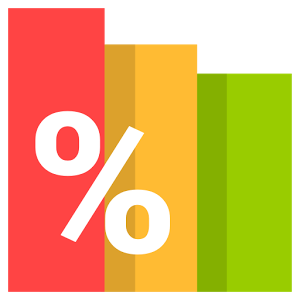
\includegraphics[scale=0.05]{A02_icon.png} & \href{https://play.google.com/store/apps/details?id=at.markushi.expensemanager}{Expense Manager} & Markus Hintersteiner \\

App 3 & 
\includegraphics[scale=0.05]{A03_icon.png} & \href{https://play.google.com/store/apps/details?id=com.bruno.myapps.droidwallet}{Droid Wallet} & William Bruno \\

App 4 & 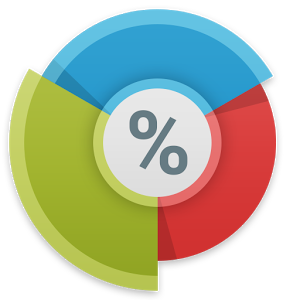
\includegraphics[scale=0.05]{A04_icon.png} & \href{https://play.google.com/store/apps/details?id=com.code44.finance}{Financius - Expense Manager} & Mantas Varnagiris \\

App 5 & 
\includegraphics[scale=0.05]{A05_icon.png} & \href{https://play.google.com/store/apps/details?id=com.handyapps.expenseiq}{Expense IQ} & Handy Apps \\

App 6 & 
\includegraphics[scale=0.05]{A06_icon.png} & \href{https://play.google.com/store/apps/details?id=com.techahead.ExpenseManager}{Diario Gasto Gerente (Daily Expense Manager)} & Gullak \\

App 7 & 
\includegraphics[scale=0.05]{A07_icon.png} & \href{https://play.google.com/store/apps/details?id=com.bookmark.money}{Money lover - Expense Manager} & ZooStudio   \\

App 8 & 
\includegraphics[scale=0.05]{A08_icon.png} & \href{https://play.google.com/store/apps/details?id=com.kpmoney.android}{AndroMoney (Expense Track)} & AndroMoney \\

App 9 & 
\includegraphics[scale=0.05]{A10_icon.png} & \href{https://play.google.com/store/apps/details?id=cz.destil.settleup}{Settle up} & David Vávra \\

App 10 & 
\includegraphics[scale=0.05]{A11_icon.png} & \href{https://play.google.com/store/apps/details?id=com.Splitwise.SplitwiseMobile}{Splitwise} & Splitwise \\

\hline
\end{tabular} 
\caption{Taula amb les aplicacions existents}
\label{fig:apps}
\end{table}

Actualment hi ha dos tipus d'aplicacions relacionades amb la gestió de despeses. Per una banda les que serveixen per enregistrar les despeses i/o ingressos personals, tot categoritzant-los (Aplicacions 1 - 8) i per l'altra les que serveixen per a gestionar despeses compartides en grup i/o deutes personals amb coneguts (Aplicacions 9 i 10).

%TODO More info about SUS. 
Per a veure el grau de satisfacció dels usuaris amb les aplicacions existents s'ha fet servir el qüestionari \gls{SUS} amb 4 usuaris. Amb els resultats s'ha fet la mitjana dels 4 usuaris per cada aplicació donant com a resultat els valors de la figura (\ref{fig:Apps_art_state}). Com es pot veure els usuaris no tenen una bona \ac{UX} al fer servir varies d'aquestes aplicacions, ja que obtenen una nota bastant baixa.

\begin{figure}[htp]
\centering
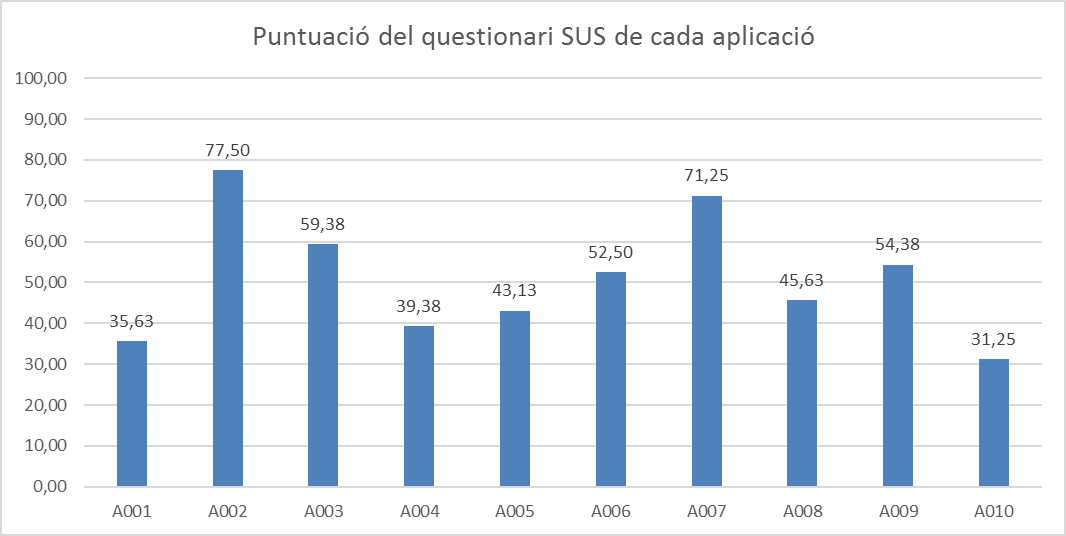
\includegraphics[scale=0.8]{Apps_art_state_SUS.png}
\caption{Puntuació de les aplicacions existents amb el questionari SUS}\label{fig:Apps_art_state}
\end{figure}

\subsection{Aplicacions per gestionar despeses en grup}



\section{Estudi de la meva app}

%mirar invision app (web per a fer dissenys)
\section{Conclusions}
\section{Agraïments}

\begin{thebibliography}{9}

%Autor / Titol (Cursiva) / Dades de la publicació
\bibitem{Android_OS}
International Data Corporation. \textit{Smartphone OS Market Share, Q2 2014}. [\url{http://www.idc.com/prodserv/smartphone-os-market-share.jsp}, 20 d'Octubre del 2014].

\bibitem{def_UX}
Rex Hartson. \textit{The UX Book: Process and Guidelines for Ensuring a Quality User Experience}. EEUU: Elseiver, 2012, p. 19.

\bibitem{cant_design_UX}
Smashing Magazine. \textit{User Experience Design}. Alemanya: Smashing Media GmbH, 2012, p. 25-28.

\bibitem{user_centred_design}
Udacity. \textit{Personas and Use Cases Interview with Rich Fulcher}. [\url{https://www.youtube.com/watch?v=uL6xlI17gBU}, 22 de Novembre del 2014]. 

\bibitem{udacity_UX}
Udacity. \textit{UX Design for Mobile Developers}. [\url{https://www.udacity.com/course/ud849}, 22 de Novembre del 2014]

\end{thebibliography}

\end{document}